\chapter{Design and Implementation}\label{ch:design-implementation}
In this chapter we overview the design of {\sys} traffic shaping tunnel. 

\section{Traffic Shaping Tunnel}

The previous section describes an abstract differentially private traffic shaping strategy.
We now present \sys's traffic-shaping tunnel.

A tunnel must address three requirements. First, it must satisfy DP guarantees. For this, the tunnel~must complete DP measurements and prepare shaped packets within each interval, and it must be able to transmit all payload bytes generated from an application within a finite window length (as defined in the DP strategy).
%
Secondly, the payload and dummy bytes in the shaped packets must be indistinguishable to an adversary.
For this, the payload and dummy bytes must be transmitted through a shared transport layer so that they are identically acknowledged by the receiver and subject to congestion control and loss recovery mechanisms.
%
Finally, the tunnel must provide similar levels of reliability, congestion control, and loss recovery as expected by the application.
\begin{figure}[t]
  \centering
  %  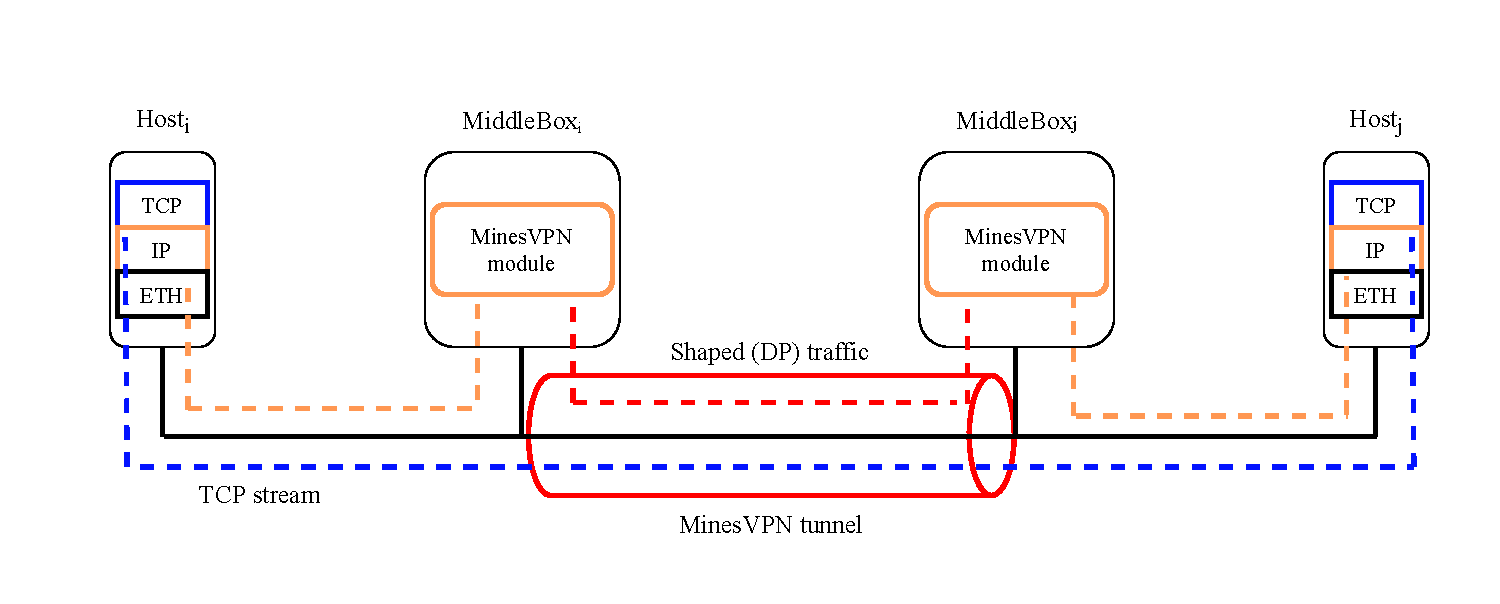
\includegraphics[width=\columnwidth]{figures/Design_highlevel.pdf}
  %  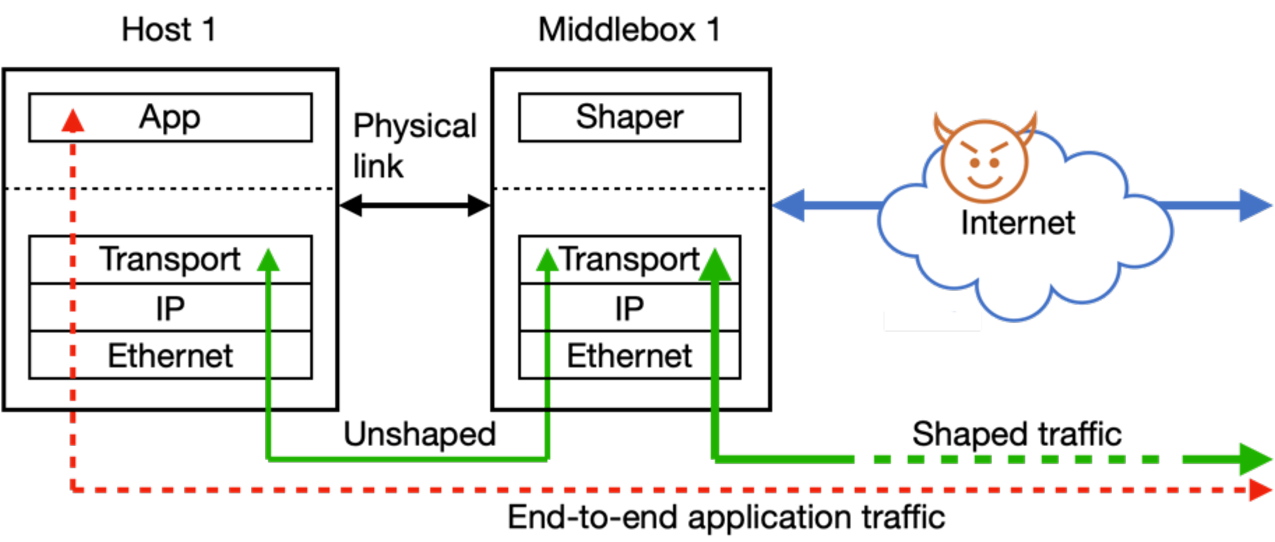
\includegraphics[width=\columnwidth]{figures/minesvpn-overview-half.pdf}
  %  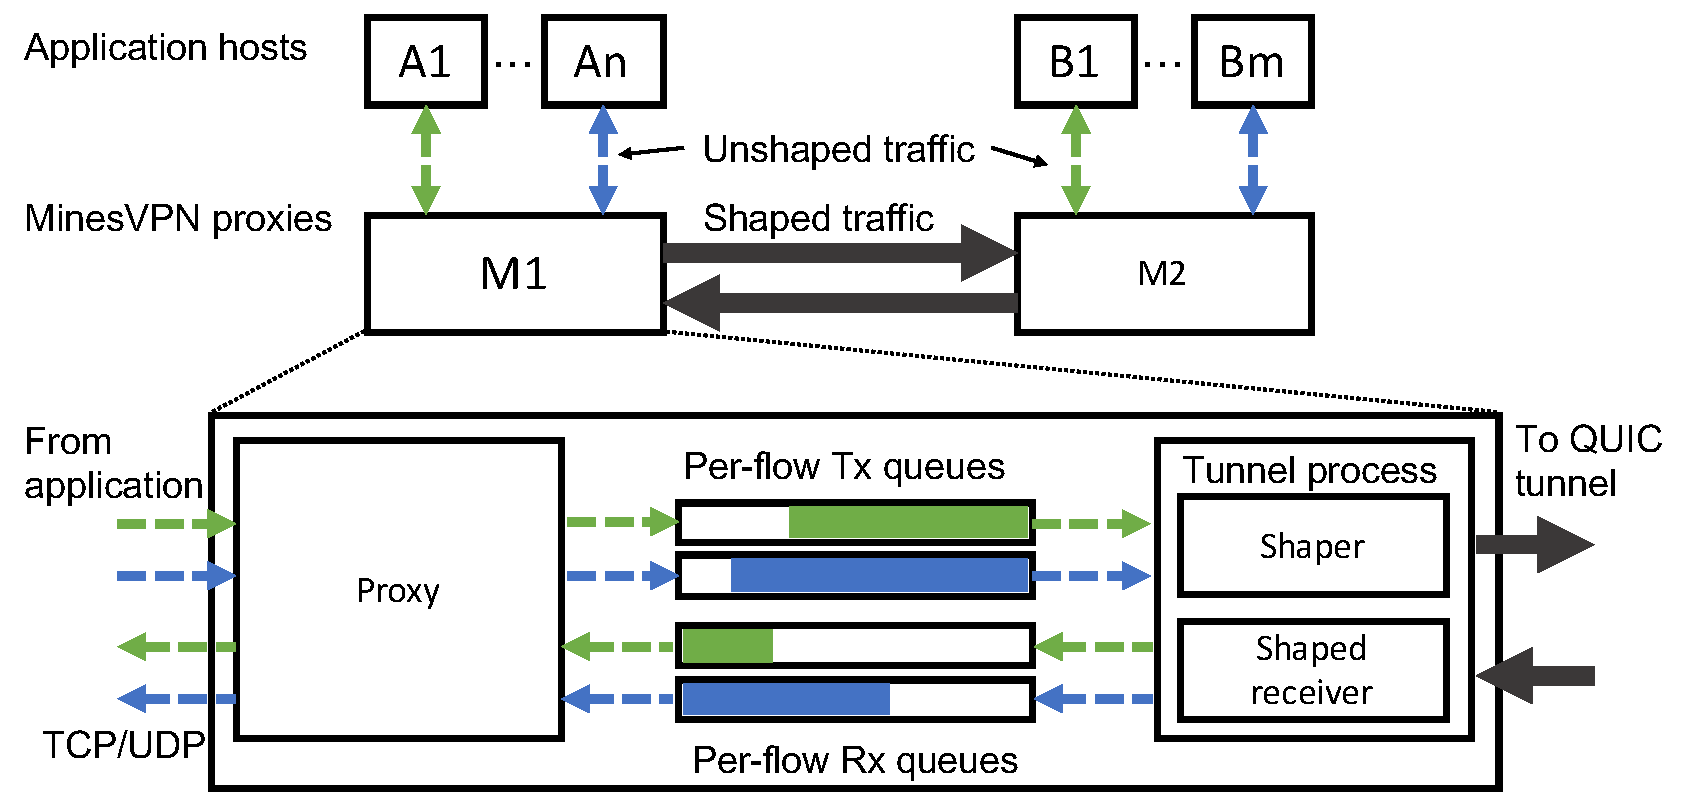
\includegraphics[width=\columnwidth]{figures/minesvpn-arch4.pdf}
  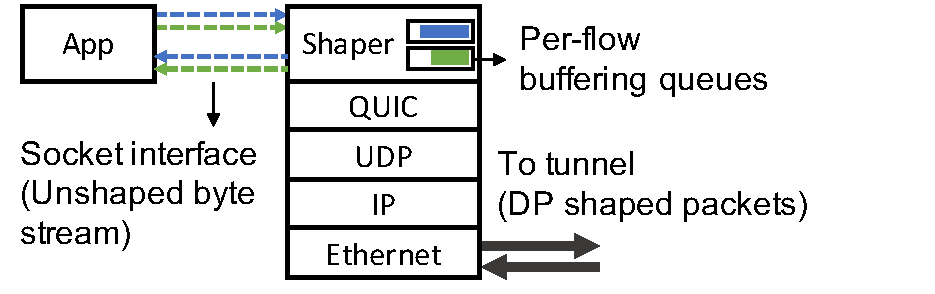
\includegraphics[width=\columnwidth]{figures/design2.pdf}
  \caption{Overview of tunnel design (one endpoint)
      %\am{Update figure}
  }
  \label{fig:minesvpn-overview}
\end{figure}

\Cref{fig:minesvpn-overview} shows the design of one endpoint of {\sys}’s traffic shaping tunnel. A similar endpoint is deployed on the other end of the tunnel.
The shape of the traffic in the tunnel can be configured independently in each direction. The privacy loss in bidirectional streams is the DP composition of the privacy loss in each direction.
A tunnel endpoint consists of a shaping layer (Shaper) on top of QUIC, which in turn runs on top of a standard UDP stack
It's worth mentioning that aside from QUIC/UDP, {\sys} has the option to utilize a conventional TCP stack as well.
The tunnel endpoints establish a bidirectional QUIC connection and generate DP-sized transmit buffers in fixed intervals, which carry payload bytes from one or more application flows.
In the absence of application payload, a tunnel endpoint transmits dummy bytes, which are discarded at the other endpoint.
QUIC encrypts all outbound packets.

{\sys} adopts a transport-layer proxy architecture: each application terminates a connection with its local tunnel endpoint.
The application byte stream is sent to the remote application over three piecewise connections: 
(i) between the application and its local tunnel endpoint,
(ii) between the tunnel endpoints, and
(iii) between the remote tunnel endpoint and the remote application.
This ensures only one active congestion control and reliable delivery mechanism in the tunnel and that all bytes are subject to identical mechanisms.
We discard tunneling TCP through TCP and use QUIC as TCP-in-TCP tunneling causes TCP meltdown~\cite{honda2005tcpovertcp, tcp-meltdown} problem.
In a TCP-in-TCP tunnel, when the network experiences packet loss, the lower-layer TCP initiates packet retransmission to ensure delivery.
However, the upper-layer TCP protocol is unaware of this packet loss and wrongly interprets the increased delay as a sign of a slow network, leading it to decrease the transmission rate.
Consequently, this slower transmission causes the lower-layer TCP protocol to receive acknowledgments too slowly, further mistaking it as packet loss within the network, and thus triggering retransmission.
This repetitive cycle creates a detrimental effect on network performance known as the TCP meltdown problem, significantly degrading overall efficiency.
The other option was to use TCP-in-UDP tunnel. 
This, however, violates the privacy guarantees of {\sys}.
In case of packet losses, the application TCP protocol retransmits data to guarantee data delivery. 
On the other hand, the dummy bytes that are injected in the traffic shaping tunnel are not retransmitted, making them observable for adversary. 
